%**************************************************************
\section{Il paradigma dichiarativo: Flutter}
\label{sec:paradigma-dichiarativo-flutter}

\textbf{N.B.} L'implementazione dell'esempio è ridotta al minimo indispensabile e come si potrà vedere dalle immagini l'applicazione sarà composta da un pulsante dell'intera grandezza della schermata.

\subsection{Creazione dell'interfaccia grafica}
\label{subsec:creazione-ui-qt}

Per implementare l'esempio indicato in "\hyperref[sec:introduzione-esempio-confronto-paradigmi]{Introduzione all'esempio per il confronto}", sono necessari un po' più widget, in quanto Flutter li usa in maniera intensa, ma il codice è decisamente meno verboso.
\begin{lstlisting}
// Widget che definisce la schermata.
// Essendo uno StatefulWidget non definisce il metodo build,
// in quanto compito del possessore dello stato, ossia
// la classe _ExampleAppState.
class ExampleApp extends StatefulWidget {
  State<ExampleApp> createState() => _ExampleAppState();
}

// Stato collegato al widget ExampleApp.
class _ExampleAppState extends State<ExampleApp> {
  // Nessun widget viene dichiarato in anticipo.
  // Solo le variabili che sono parte dello stato
  // vanno dichiarate.
  final random = new Random();
  int r;
  
  // Questo metodo indica cosa va fatto ogni volta
  // che lo stato di ExampleApp viene creato da zero.
  @override
  void initState() {
    super.initState();
    r = random.nextInt(10);
  }

  // Callback che viene passata ad onPressed.
  // Corrisponde allo slot privato di ExampleApp 
  // in Qt chiamato buttonClicked.
  void _buttonClicked() {
    setState(() => r = random.nextInt(10));
  }

  // Questo metodo indica che cosa mostrare a schermo.
  // Notare come i concetti di Element e RenderObject
  // non sono presenti, in quanto sono onere di Flutter.
  @override
  Widget build(BuildContext context) {
    // MaterialApp, paragonabile a QApplication.
    return MaterialApp(
      // RaisedButton, paragonabile a QPushButton.
      home: RaisedButton(
        // In Flutter il campo dati child di un widget ha sempre 
        // tipo Widget. Quindi un pulsante non contiene solo 
        // testo, ma anche qualsiasi altra cosa (in questo
        // caso, semplice testo).
        child: Text("Generato: $r"),
        // Definizione del callback da invocare
        // alla pressione del pulsante.
        onPressed: _buttonClicked,
      ),
    );
  }
}
\end{lstlisting}
Riassumendo, nella classe \texttt{ExampleApp}, che estende \texttt{StatefulWidget}, viene:
\begin{itemize}
    \item definito il widget e siccome ha uno stato, viene creato lo stato correlato;
    \item dato che lo stato del widget interessa solo a \texttt{ExampleApp}, viene dichiarato privato (al di fuori del file non è visibile);
    \item generato il valore di $r$ iniziale in \texttt{initState};
    \item impostato nel metodo \texttt{build} che cosa viene visualizzato quando il widget viene costruito (definito $state$, \texttt{build} definisce $f(state)$);
    \item dichiarato che cosa deve avvenire all'evento di pressione del pulsante.
\end{itemize}
Quello che succede alla pressione del pulsante è la generazione di un evento \emph{onPressed} che richiama il \emph{callback} (metodo \texttt{\_buttonClicked}). All'interno del \emph{callback} ci si è occupati solo di aggiornare $r$ e di indicare che il widget va ricostruito con \texttt{setState}.

\subsection{Creazione del punto di ingresso}
\label{subsec:creazione-main-qt}

Oltre alla definizione di \texttt{ExampleApp}, va definita la funzione \texttt{main}, il punto d'ingresso del programma:
\begin{lstlisting}
import 'package:flutter/material.dart';
import 'dart:math';

void main() => runApp(ExampleApp());
\end{lstlisting}
Quello che avviene in questo \texttt{main} è inserire come widget radice nel \emph{Widget tree} un'istanza di \texttt{ExampleApp}. Visto che il \texttt{main} dispone di una sola istruzione è stato possibile usare la \emph{arrow notation}.\\
L'applicazione realizzata è la seguente:
\begin{figure}[!h] 
  \centering 
  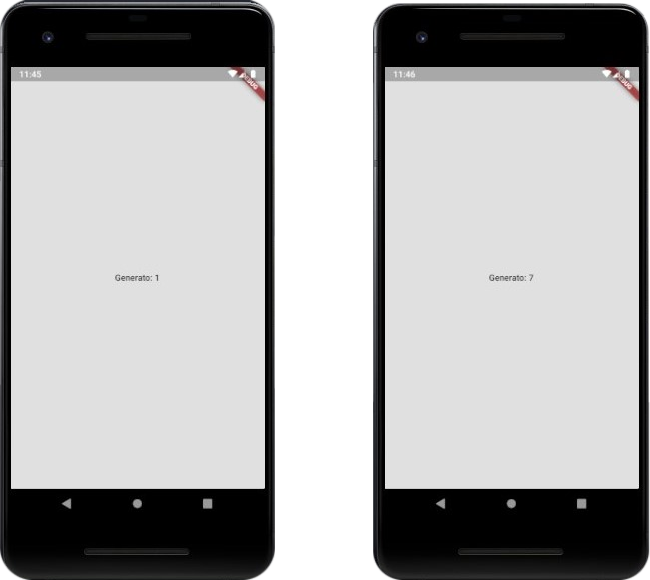
\includegraphics[width=1.0\columnwidth]{capitolo-5/flutter} 
  \caption{Esempio in Flutter - Applicazione prima (sinistra) e dopo (destra) la pressione del pulsante}
\end{figure}

\subsection{Osservazioni sul procedimento}
\label{subsec:osservazioni-procedimento-qt}

Quello che si può notare subito è la minor verbosità, sotto certi aspetti (per esempio non è necessario dichiarare che il widget va mostrato a schermo, non bisogna connettere eventi e \emph{callback} in separata sede).\\
Ma ciò che veramente conta è la separazione dei concetti.
La costruzione dell'interfaccia, basata sullo stato, è svolta solamente nel metodo \emph{build}. L'aggiornamento dello stato, svolto da \texttt{\_buttonClicked} a riga 29 di \texttt{ExampleApp}, è una pura operazione di aggiornamento stato.
Anche volendo creare un'istanza di \texttt{RaisedButton} all'esterno del metodo \texttt{build} (tecnicamente possibile) e accedendovi da dentro \texttt{\_buttonClicked}, non si sarebbe in grado di far alcuna modifica perché \texttt{RaisedButton} è un widget, e i widget sono per definizioni immutabili.
Solo richiamando \texttt{setState} è possibile informare il corrispondente \texttt{Element} che il \texttt{RenderObject} del widget va aggiornato, causando l'aggiornamento della schermata.